\documentclass{ximera}  
\title{Flowcharts}  
\begin{document}  
\begin{abstract}  
We introduce flowcharts as a way to organize a procedure designed to solve a particular problem.
\end{abstract}  
\maketitle

An algorithm is a fixed set of instructions that can be followed to solve a problem. Algorithms take in a set of inputs from a predefined set, perform a series of clearly defined computations, and produce an output meant to solve a particular problem. While it may take a while for an algorithm to produce an answer (say, if the size of the input is large), it should always be the case that the solution to the problem is found in a finite amount of time.


There are several ways to specify an algorithm. For now we will represent our algorithms using a special type of diagram known as a flowchart. As we gain more experience we will be able to transition to other methods for expressing algorithms. We begin with flowcharts because they are a relatively intuitive to use and because you probably have some prior experience with them.

Here, for example, are two different algorithms for accomplishing the same task. 

\begin{center}
	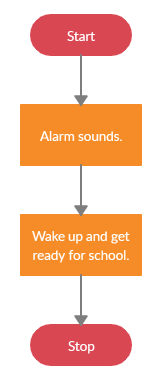
\includegraphics{morning1.png}
\end{center}
\begin{center}
	An example of an algorithm for your morning routine.
\end{center}

\begin{center}
	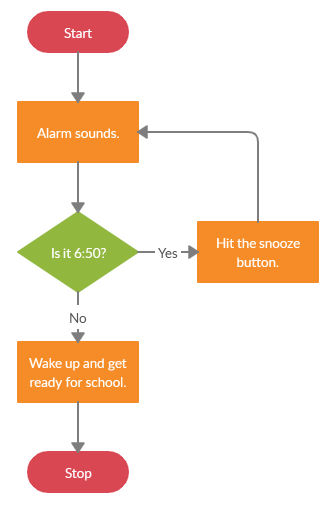
\includegraphics{morning2.png}
\end{center}
\begin{center}
	Another example of an algorithm for your morning routine.
\end{center}

We use the following conventions for our flowchart compartments (there are others, but these are the main ones we will use). Arrows between the different compartments show how the algorithm progresses from one operation/input/decision to another.

\begin{center}
	
\includegraphics{startstop.png}
\end{center}
\begin{center}
	Beginning or end of the algorithm.
\end{center}

\begin{center}
	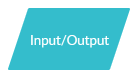
\includegraphics{io.png}
\end{center}
\begin{center}
	Indicates data input or output.
\end{center}

\begin{center}
	
\includegraphics{decision.png}
\end{center}
\begin{center}
	Conditional operation/decision. Typically limited to true/false or yes/no options.
\end{center}

\begin{center}
	
\includegraphics{process.png}
\end{center}
\begin{center}
	A set of operations.
\end{center}

We can use a simple algorithm to compute the absolute value of any real number $x$.

\begin{center}
	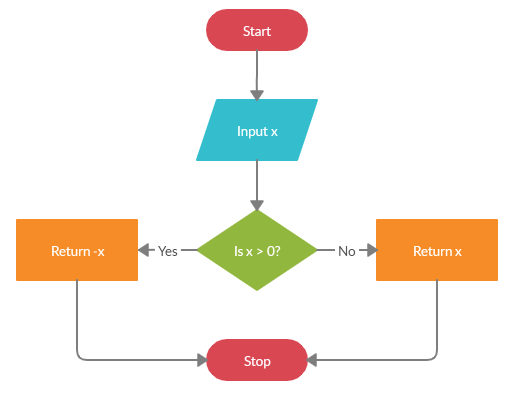
\includegraphics{absalgo.png}
\end{center}
\begin{center}
	An example of an algorithm that computes $|x|$.
\end{center}

\begin{problem}
	Consider the following scenario. Suppose that you can buy an avocado at the grocery store for \$1 or 5 avocados for \$3. Develop an algorithm for computing the minimum price for buying $n$ avocados where $1\leq n\leq 5$ and draw a flowchart for your algorithm.
	\begin{hint}
		You can modify the algorithm for computing $|x|$. Note that the second hint for this problem is the solution.
	\end{hint}
	\begin{hint}
		\begin{center}
			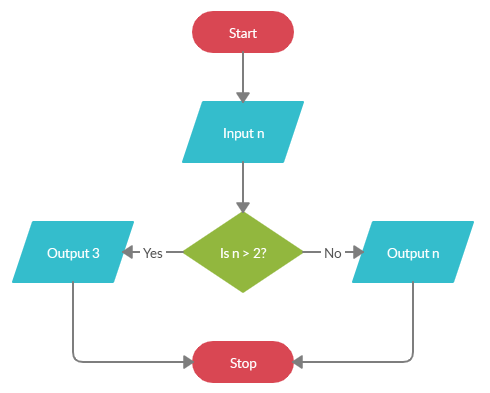
\includegraphics{avocados.png}
		\end{center}
	\end{hint}
\end{problem}
\end{document}
